\chapter{Méthodologie d'étude et besoins du projet}
\label{chap:deux}

Ce chapitre expose la démarche suivie. Il précise la nature de l'étude et les modalités de collecte des données, puis caractérise le jeu de données constitué, en particulier sous l'angle de sa qualité et de ses biais. Il formalise ensuite les besoins du projet, les priorise, définit les livrables attendus et évalue les risques identifiés.

\section{Méthodologie d'étude}
\label{sec:2-1}

\subsection{Nature de l'étude}

L'étude relève de la \textbf{recherche-action}. Trois caractéristiques du travail conduit le justifient : elle porte sur une situation observée dans son contexte réel et non sur un dispositif expérimental ; elle associe la production de connaissance sur le fonctionnement de la structure à la conception d'une intervention destinée à en modifier les pratiques ; elle est conduite en interaction avec les acteurs concernés, dont les observations ont orienté les choix de conception.

Cette démarche mobilise quatre approches complémentaires : \textbf{descriptive}, pour établir un état des pratiques de gestion de l'information en vigueur ; \textbf{exploratoire}, pour identifier les difficultés et les besoins dans un contexte peu documenté ; \textbf{quantitative}, appliquée au jeu de données constitué, pour mesurer les anomalies et produire les indicateurs ; et \textbf{qualitative}, fondée sur l'observation directe et les échanges avec le personnel, pour comprendre les pratiques et leurs raisons.

\subsection{Collecte de données}

\subsubsection{Objectifs de la collecte}

La collecte poursuivait trois objectifs : caractériser les processus de gestion de l'information en vigueur ; constituer un jeu de données exploitable à partir des supports existants ; et identifier les besoins des différents acteurs de la structure.

\subsubsection{Sources de données étudiées}

Les sources exploitées sont énumérées au tableau~\ref{tab:sources}. Une précision s'impose sur leur hiérarchie, car elle conditionne la reproductibilité de tous les chiffres avancés dans ce rapport.

\textbf{L'état des ventes du VARBAF fait foi.} Ce classeur, tenu par la structure et arrêté au 25~février~2026, constitue la source primaire : tout chiffre relatif aux ventes, aux commissions, aux reversements et à la caisse en est directement calculé, et non repris d'un traitement intermédiaire. Le relevé du parc locatif n'intervient qu'à deux titres, l'un et l'autre signalés à chaque usage : il fournit l'état de recouvrement des redevances, absent du classeur, et il sert de référentiel au rattachement des noms d'artisans à des espaces. Lorsqu'une valeur produite par le système diverge d'une valeur du classeur, c'est le classeur qui prévaut et l'écart qui est signalé.

\begin{table}[H]
\centering
\caption{Sources de données exploitées}
\label{tab:sources}
\singlespacing
\begin{tabularx}{\textwidth}{@{}p{3.4cm}p{2.1cm}X@{}}
\toprule
\entete{Source} & \entete{Nature} & \entete{Contenu}\\
\midrule
Registre des dépôts et ventes & Manuscrit & Dépôts de produits, annotation de vente, nom de l'artisan, observation de décharge, reste à payer ; transcrit depuis mai 2024, exploité sur l'exercice 2026\\
État des ventes --- feuille \emph{Ventes} & Tableur & Reprise informatique du registre : 603 lignes, avec sous-totaux mensuels\\
État des ventes --- feuille \emph{Commissions} & Tableur & 95 décharges de reversement datées, avec montant de vente et commission retenue\\
État des ventes --- feuille \emph{Caisse} & Tableur & Comptage des espèces par coupure, avoirs dus, différence constatée, sorties postérieures\\
État des ventes --- feuille \emph{Récapitulatif} & Tableur & Campagne de reversement préparée : bénéficiaires, montants, commission, net à percevoir\\
Relevé des occupants & Tableur & Occupants, espaces attribués, secteurs, redevances mensuelles, suivi du recouvrement 2026\\
Inventaire des produits & Tableur & Désignation, secteur, matériaux, conditionnement, capacité, prix unitaire, artisan\\
Échanges avec le personnel & Oral & Fonctionnement des sections, processus, difficultés rencontrées\\
Observation directe & Terrain & Déroulement des opérations de dépôt, de vente et d'encaissement\\
\bottomrule
\end{tabularx}
\onehalfspacing
\source{élaboré par l'auteur.}
\end{table}

\subsubsection{Modalités de collecte}

L'observation directe a porté sur les activités quotidiennes, en particulier les dépôts de produits et les ventes au comptoir ; elle a permis d'établir la séquence effective des gestes et des enregistrements, qui diffère parfois de la procédure théorique. L'analyse documentaire a consisté en la transcription du registre manuscrit en format tabulaire et en l'extraction, la normalisation et la confrontation des classeurs de suivi. Les échanges avec les responsables ont porté sur le fonctionnement des sections et sur les difficultés rencontrées dans l'exercice de leurs missions.

\subsubsection{Processus étudiés}

L'observation a porté en priorité sur deux processus, dont la description figure ci-après.

Le \textbf{processus d'attribution d'un espace} se déroule en trois étapes. L'artisan constitue d'abord un dossier de demande, comprenant une demande timbrée adressée au Coordonnateur, une attestation d'enregistrement dans sa commune d'activité, des images des œuvres ou produits à exposer, le plan de localisation de son atelier de production et une photocopie de sa pièce d'identité. Le dossier est ensuite examiné et validé par le Coordonnateur, qui attribue un espace. L'artisan bénéficie enfin d'un premier mois gratuit, avant de s'acquitter d'une redevance mensuelle.

Le \textbf{processus de dépôt et de vente} s'articule autour du registre. L'artisan confie ses produits au village, qui les inscrit avec leur désignation, leur conditionnement, leur quantité et leur prix unitaire, ce dernier étant fixé par l'artisan lui-même. Les produits sont validés par la section Production avant exposition. Lorsqu'une vente intervient, elle est signalée par une annotation en regard de la ligne de dépôt. En cas de rupture de stock, les sections Production et Commercialisation contactent l'artisan pour réapprovisionnement.

\begin{figure}[H]
\centering
\begin{tikzpicture}[
  font=\footnotesize,
  etape/.style={draw,rounded corners=2pt,align=center,text width=2.6cm,minimum height=11mm,fill=black!5},
  doc/.style={draw,align=center,text width=2.4cm,minimum height=9mm,fill=black!10},
  fl/.style={-{Latex[length=2mm]},thick}]

\node[etape] (a) {Artisan\\confie ses produits};
\node[etape,right=8mm of a] (b) {Inscription\\au registre};
\node[etape,right=8mm of b] (c) {Validation\\section Production};
\node[etape,right=8mm of c] (d) {Exposition\\en boutique};
\node[etape,below=9mm of d] (e) {Vente\\au comptoir};
\node[doc,left=8mm of e] (f) {Annotation\\en regard\\de la ligne};
\node[etape,left=8mm of f] (g) {Reversement\\à l'artisan};

\draw[fl] (a) -- (b); \draw[fl] (b) -- (c); \draw[fl] (c) -- (d);
\draw[fl] (d) -- (e); \draw[fl] (e) -- (f); \draw[fl] (f) -- (g);

\node[font=\scriptsize\itshape,align=center,below=2mm of f,text width=4.4cm,black!65]
 {la vente n'a pas d'enregistrement propre :\\c'est ici que la traçabilité se perd};
\end{tikzpicture}
\caption{Processus de dépôt et de vente tel qu'observé sur le terrain}
\source{élaboré par l'auteur d'après l'observation directe.}
\end{figure}

\section{Variables, indicateurs et données de l'étude}
\label{sec:2-2}

\subsection{Variables retenues et leur nature}

Le tableau~\ref{tab:variables} récapitule les variables exploitées, leur nature statistique et leur source.

\begin{table}[H]
\centering
\caption{Variables de l'étude, nature et source}
\label{tab:variables}
\singlespacing
\begin{tabularx}{\textwidth}{@{}p{3.4cm}p{3.6cm}X@{}}
\toprule
\entete{Variable} & \entete{Nature} & \entete{Source et remarque}\\
\midrule
Désignation du produit & Qualitative nominale & Registre ; porte souvent le conditionnement dans le libellé\\
Type d'artisanat & Qualitative nominale & Registre ; deux modalités, art et production\\
Montant de la vente & Quantitative continue & Registre ; seule valeur monétaire inscrite\\
Quantité et prix unitaire & Quantitatives & \emph{Non inscrits} ; déduits du montant\\
Nom de l'artisan & Qualitative nominale & Registre ; écriture libre, plusieurs formes par personne\\
Observation de décharge & Qualitative nominale & Registre ; trace du reversement, texte libre\\
Reste à payer & Quantitative continue & Registre ; part artisan non encore reversée\\
Espace locatif & Qualitative nominale & Relevé du parc ; obtenu par rapprochement du nom\\
Redevance mensuelle & Quantitative continue & Relevé du parc ; montant convenu, de 2 000 à 60 000 F\\
\bottomrule
\end{tabularx}
\onehalfspacing
\source{élaboré par l'auteur.}
\end{table}

Trois de ces variables appellent un commentaire.

Le \textbf{conditionnement} n'existe pas comme colonne : il est porté dans la désignation elle-même --- \guillemotleft~savon 1~l~\guillemotright, \guillemotleft~miel 650~g~\guillemotright{} --- de sorte qu'un même produit vendu en plusieurs formats apparaît sous plusieurs désignations à des prix différents. Le miel est ainsi commercialisé entre 1~500 et 8~500~francs~CFA. Cette configuration a une conséquence directe sur la modélisation, exposée à la section~\ref{sec:3-3-4}.

La \textbf{redevance mensuelle} s'échelonne de 2~000 à 60~000~francs~CFA sans relation avec la superficie occupée, ce qui écarte l'hypothèse d'un tarif au mètre carré et conduit à la modéliser comme un montant convenu, propre à chaque attribution et figé sur le contrat. Ce point mérite d'être signalé, car l'hypothèse contraire avait initialement été retenue par déduction : un tarif au mètre carré est cohérent sur le papier et se rencontre dans les modèles de référence, mais il n'a jamais produit un seul montant, faute de barème existant au village.

L'\textbf{observation de décharge} porte la trace du reversement, rédigée en clair et sans format imposé : \guillemotleft~Payé le 19/02/2026 à Mme Guessong~\guillemotright, ou une simple date. Elle constitue la seule preuve du paiement de l'artisan dans le dispositif actuel. Une transcription antérieure l'avait interprétée comme portant l'identité du vendeur, au motif qu'un nom de personne y figure fréquemment ; le rapprochement avec la feuille des commissions établit qu'il s'agit du bénéficiaire ou de l'intermédiaire d'une décharge. L'identité du vendeur n'est en réalité enregistrée nulle part : c'est une information que le système proposé introduit, non une information qu'il reprend.

\subsection{Description du jeu de données}

\subsubsection{Corpus transcrit et période d'analyse}

Il convient de distinguer deux ensembles que la suite du rapport ne confond jamais.

Le \textbf{corpus transcrit} compte 603~lignes de registre, remontant à mai~2024. Il constitue ce qui a été saisi et ce que le système contient. Sa reprise complète est décrite au chapitre~3, et le rapport d'import produit à cette occasion en donne les caractéristiques d'ensemble.

La \textbf{période d'analyse} est le seul exercice~2026. Tous les indicateurs présentés dans ce rapport, sans exception, portent sur cette période. Le motif est exposé à la délimitation temporelle de l'introduction et se résume ainsi : le relevé de recouvrement n'existe que pour 2026, et les défauts de datation du registre se concentrent intégralement sur les exercices antérieurs. Faire porter un indicateur sur une période dont une source est absente ne produit pas un indicateur partiel mais un indicateur faux.

Sur l'exercice 2026, le jeu retenu compte 195~lignes de vente couvrant janvier à juin, 36~espaces locatifs relevés sur 18~contenants, 21~artisans identifiés et 130~désignations de produits distinctes. Les formats d'origine sont manuscrits pour le registre et tabulaires pour les deux classeurs de suivi.

Le chiffre d'affaires de la période s'élève à 791~400~francs~CFA, dont 79~140~francs~CFA de commission au taux de 10~\% en vigueur et 712~260~francs~CFA de part revenant aux artisans.

\begin{figure}[H]
\centering
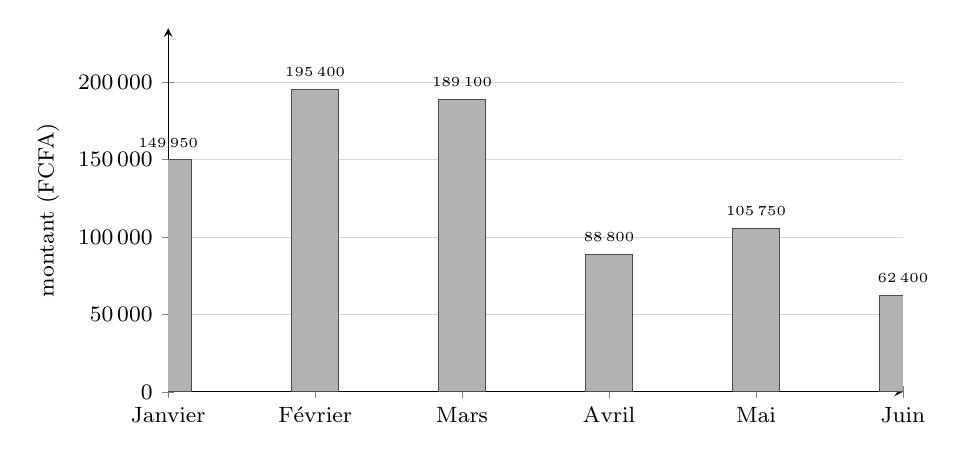
\begin{tikzpicture}
\begin{axis}[
  width=0.9\textwidth, height=6.2cm,
  ybar, bar width=17pt, enlarge x limits=0.13,
  ymin=0, ymax=235000,
  ylabel={\footnotesize montant (FCFA)},
  symbolic x coords={Janvier,Février,Mars,Avril,Mai,Juin},
  xtick=data,
  scaled y ticks=false,
  ytick={0,50000,100000,150000,200000},
  yticklabels={0,50\,000,100\,000,150\,000,200\,000},
  yticklabel style={font=\footnotesize},
  tick label style={font=\footnotesize},
  label style={font=\footnotesize},
  ymajorgrids, grid style={black!15},
  nodes near coords,
  every node near coord/.append style={font=\tiny,yshift=1pt,
     /pgf/number format/fixed,/pgf/number format/1000 sep={\,}},
  axis lines=left]
\addplot[fill=black!30,draw=black!70] coordinates
  {(Janvier,149950)(Février,195400)(Mars,189100)(Avril,88800)(Mai,105750)(Juin,62400)};
\end{axis}
\end{tikzpicture}
\caption{Chiffre d'affaires mensuel, exercice 2026}
\label{fig:camensuel}
\source{calculé par l'auteur à partir du registre transcrit.}
\end{figure}

Le fléchissement du mois de juin s'explique par la clôture de la transcription en cours de mois et ne traduit pas une baisse d'activité. La lecture des cinq premiers mois fait en revanche apparaître un repli net à partir d'avril, dont les données disponibles ne permettent pas d'établir la cause : elle peut tenir à la saisonnalité de la fréquentation comme à un relâchement de la tenue du registre. Distinguer les deux supposerait précisément l'instrument que le présent travail met en place.

\subsubsection{Répartition par type d'artisanat}

Le registre classe chaque vente selon deux catégories, l'artisanat d'art et l'artisanat de production. Cette colonne est renseignée sur la totalité des lignes de 2026 et pratiquement absente des exercices antérieurs --- 389~lignes vides sur 392 en 2025, 14 sur 16 en 2024 --- ce qui constitue un argument supplémentaire, et le plus net, en faveur de la restriction retenue.

\begin{table}[H]
\centering
\caption{Répartition des ventes par type d'artisanat, exercice 2026}
\label{tab:typeartisanat}
\singlespacing
\begin{tabularx}{\textwidth}{@{}Xrrrr@{}}
\toprule
\entete{Type d'artisanat} & \entete{Lignes} & \entete{Montant (FCFA)} & \entete{Part} & \entete{Reste à payer}\\
\midrule
Artisanat d'art & 70 & 546 250 & 69,0 \% & 164 700\\
Artisanat de production & 125 & 245 150 & 31,0 \% & 62 150\\
\midrule
\textbf{Total} & \textbf{195} & \textbf{791 400} & \textbf{100,0 \%} & \textbf{226 850}\\
\bottomrule
\end{tabularx}
\onehalfspacing
\source{calculé par l'auteur à partir de l'état des ventes du VARBAF.}
\end{table}

Cette répartition présente une inversion qu'il faut relever. L'artisanat de production concentre 64,1~\% des transactions mais seulement 31,0~\% du chiffre d'affaires ; l'artisanat d'art fait l'inverse. La distribution des montants le confirme : le panier moyen s'établit à 4~058~francs~CFA pour une médiane de 1~500~francs~CFA, dans une amplitude allant de 100 à 107~000~francs~CFA.

Une moyenne près de trois fois supérieure à la médiane signale une distribution fortement dissymétrique, où quelques ventes d'objets d'art portent l'essentiel du chiffre d'affaires tandis que le flux quotidien est constitué de produits agroalimentaires de faible valeur unitaire. Cette structure a une conséquence de gestion : le suivi du chiffre d'affaires ne renseigne pas sur l'activité du village, et réciproquement. Le tableau de bord présenté au chapitre~3 restitue en conséquence le montant et le nombre de ventes comme deux indicateurs distincts, jamais l'un à la place de l'autre.

\subsubsection{Qualité}

L'analyse du jeu de données met en évidence quatre catégories d'anomalies, quantifiées au tableau~\ref{tab:qualite}.

La première tient à l'\textbf{incomplétude des valeurs élémentaires}. Aucune des 195~lignes de 2026 ne porte les trois valeurs quantité, prix unitaire et montant ; la quantité est systématiquement absente et doit être déduite des deux autres. Le registre porte en effet le seul montant, la quantité étant implicite lorsqu'elle vaut un. Cette déduction est légitime tant que deux valeurs sur trois sont présentes ; une ligne trop lacunaire pour être reconstituée a été rejetée plutôt que complétée par une hypothèse.

La deuxième tient à l'\textbf{impossibilité de rattacher une vente au parc locatif}, et c'est le résultat le plus lourd de conséquences. 41~lignes, soit 21,0~\% des ventes de la période, portent un nom d'artisan qui ne correspond à aucun occupant d'un espace locatif. Ces lignes représentent 159~700~francs~CFA, c'est-à-dire 20,2~\% du chiffre d'affaires de l'exercice.

Il importe de nommer exactement ce qui manque. Le nom du bénéficiaire est présent sur la totalité des lignes de 2026 ; c'est le lien avec le parc qui fait défaut. Le tableau~\ref{tab:nonrattaches} détaille les huit écritures concernées.

\begin{table}[H]
\centering
\caption{Ventes 2026 non rattachables à un espace locatif}
\label{tab:nonrattaches}
\singlespacing
\begin{tabularx}{\textwidth}{@{}Xrp{6.4cm}@{}}
\toprule
\entete{Écriture au registre} & \entete{Montant (FCFA)} & \entete{Situation}\\
\midrule
Mme Justina & 93 000 & Vend des tableaux de décoration ; aucun espace enregistré à son nom\\
VARBamenda & 32 000 & Village artisanal de Bamenda : acheteur institutionnel, non artisan installé\\
SOLISTA & 12 200 & Déposant sans contrat de location\\
Ngassam Olivier & 9 000 & Homonymie possible avec un occupant, non tranchée\\
Titi Bio & 7 500 & Déposant sans contrat de location\\
Madi cosmétique & 3 000 & Déposant sans contrat de location\\
KEMTA & 2 500 & Déposant sans contrat de location\\
Ets SAYA Désiré & 500 & Déposant sans contrat de location\\
\midrule
\textbf{Total} & \textbf{159 700} & \textbf{20,2 \% du chiffre d'affaires 2026}\\
\bottomrule
\end{tabularx}
\onehalfspacing
\source{calculé par l'auteur par rapprochement du registre et du relevé du parc locatif.}
\end{table}

Ces lignes ne sont pas écartées : la vente a eu lieu et son montant compte. Elles sont conservées avec le nom porté au registre, sans rattachement inventé à un espace. Le chiffre d'affaires demeure ainsi exact tandis que le défaut de rattachement reste explicite et chiffré.

Deux cas au moins ne relèvent pas d'un défaut de saisie mais d'une question de fond que le code ne peut pas trancher. VARBamenda est un village acheteur et non un artisan : le rattacher à un espace serait une erreur de modélisation. Mme Justina, avec 93~000~francs~CFA sur l'exercice, est soit une artisane installée dont l'attribution n'a pas été enregistrée, soit une déposante non installée --- deux situations que le système représente différemment. Ces points ont été adressés à la coordination et figurent en annexe~E avec l'hypothèse retenue à défaut de réponse.

La troisième tient à la \textbf{multiplicité des désignations}. Un même artisan apparaît sous plusieurs formes selon les sources : nom commercial, nom de personne physique, forme abrégée ou variante orthographique. Les ventes de 2026 portent 33~écritures distinctes pour 21~identités réelles. Sur l'ensemble du corpus transcrit, le rapprochement automatique au-dessus d'un seuil de similarité de 85~\% a regroupé 10~écritures sur 55, soit 18,2~\%.

La quatrième tient à des \textbf{écarts internes non expliqués} sur les deux documents financiers.

Sur le relevé de recouvrement, la somme des montants acquittés et des restes à recouvrer s'établit à 2~324~000~francs~CFA, pour une imputation annuelle de 2~478~000~francs~CFA, soit un écart de 154~000~francs~CFA.

Sur la situation de caisse, la différence entre les avoirs dus et les espèces détenues s'élève à 162~525~francs~CFA. Elle fait l'objet de la section~\ref{sec:2-2-5}.

Ces écarts sont signalés plutôt que corrigés : rien dans les données ne permet de déterminer quel terme est fautif, et un rapport qui les corrigerait en silence effacerait précisément le constat qui justifie le travail.

\begin{table}[H]
\centering
\caption{Indicateurs de qualité du jeu de données, exercice 2026}
\label{tab:qualite}
\singlespacing
\begin{tabularx}{\textwidth}{@{}Xrr@{}}
\toprule
\entete{Indicateur} & \entete{Valeur} & \entete{Part}\\
\midrule
Lignes de vente retenues (janvier à juin 2026) & 195 & 100,0 \%\\
Lignes dont la quantité a été déduite du montant et du prix & 195 & 100,0 \%\\
Lignes sans code de boutique, donc sans artisan rattachable & 41 & 21,0 \%\\
Montant correspondant, non attribuable à un artisan & \multicolumn{2}{r}{159 700 FCFA (20,2 \%)}\\
Lignes portant un nom d'artisan, un montant et un type d'artisanat & 195 & 100,0 \%\\
Lignes portant une observation de décharge & 122 & 62,6 \%\\
Lignes portant un reste à payer non nul & 73 & 37,4 \%\\
Écritures d'artisan distinctes & 33 & ---\\
Identités réelles correspondantes & 21 & ---\\
Désignations de produits distinctes & 130 & ---\\
Espaces locatifs mouvementés & 21 & ---\\
Espaces locatifs relevés au parc & 36 & ---\\
Écart interne du relevé de recouvrement & \multicolumn{2}{r}{154 000 FCFA}\\
\bottomrule
\end{tabularx}
\onehalfspacing
\source{calculé par l'auteur à partir du registre transcrit et du rapport d'import du système.}
\end{table}

À titre de repère sur l'ensemble du corpus transcrit, le rapport d'import fait état de 603~lignes traitées, 602~importées et une rejetée pour insuffisance de valeurs, ainsi que de 100~lignes dont la date a dû être reprise de la ligne précédente --- toutes antérieures à 2026. Ces chiffres caractérisent la reprise de données décrite au chapitre~3 ; ils ne fondent aucun indicateur du présent rapport.

\subsubsection{Indicateur de recouvrement}

Le relevé des occupants permet d'établir l'indicateur central de cette étude, présenté au tableau~\ref{tab:recouvrement}.

\begin{table}[H]
\centering
\caption{Recouvrement des redevances des espaces locatifs, exercice 2026}
\label{tab:recouvrement}
\singlespacing
\begin{tabularx}{0.86\textwidth}{@{}Xr@{}}
\toprule
\entete{Élément} & \entete{Montant (FCFA)}\\
\midrule
Imputation annuelle attendue & 2 478 000\\
Montant effectivement acquitté & 365 000\\
Reste à recouvrer & 1 959 000\\
Écart interne non expliqué & 154 000\\
\midrule
\textbf{Taux de recouvrement} & \textbf{14,73 \%}\\
\bottomrule
\end{tabularx}
\onehalfspacing
\source{calculé par l'auteur à partir du relevé de recouvrement 2026 du VARBAF.}
\end{table}

Ce taux appelle une précaution de lecture. Il est calculé sur la somme des imputations portées ligne à ligne, et non sur un total déclaré ; l'écart interne de 154~000~francs~CFA signalé ci-dessus interdit de retenir les trois totaux du relevé comme mutuellement cohérents. La valeur retenue est donc celle que reproduit le système à partir des données saisies, et c'est à ce titre qu'elle est opposable.

\subsubsection{Biais}

Deux biais affectent le jeu de données et doivent être signalés.

Le premier tient à la \textbf{variabilité de la tenue du registre}. Le niveau de détail dépend de la personne qui en a la charge : la mention du corps de métier, la forme du nom de l'artisan et la rédaction de l'observation de décharge varient d'une période à l'autre sans qu'aucune règle n'ait changé. Cette variabilité constitue en soi un résultat de l'étude, puisqu'elle illustre la dépendance de la qualité de l'information aux pratiques individuelles.

Le second tient à la \textbf{sélection des pages transcrites}. La transcription porte sur un ensemble de pages et non sur l'intégralité du registre. Les pages ont été retenues de manière à couvrir l'ensemble de la période, sans procédure d'échantillonnage aléatoire. Les résultats quantitatifs présentés valent donc pour l'échantillon considéré et ne peuvent être extrapolés sans précaution.

Un troisième point relève moins du biais que de la portée. La restriction à l'exercice~2026 réduit l'effectif à 195~lignes et interdit toute comparaison interannuelle. Cette perte est assumée : elle est le prix de la cohérence entre les trois sources, et une comparaison entre un exercice documenté et un exercice qui ne l'est pas produirait une variation dont rien ne dirait si elle mesure l'activité ou la qualité de la tenue du registre.

\subsubsection{Aspects éthiques}

Le relevé des occupants comporte les numéros de téléphone personnels des artisans. Ces données ont été écartées du traitement et ne figurent ni dans le jeu de données constitué, ni dans les traitements ultérieurs, ni dans les annexes du présent rapport.

La publication d'informations relatives à un artisan sur un portail accessible au public suppose son consentement. Une autorisation de publication est en conséquence portée sur la fiche de chaque artisan et conditionne son affichage. Les données financières relatives à un artisan --- ventes, soldes, reversements --- demeurent accessibles au seul personnel habilité et à l'artisan concerné.

\subsection{Le circuit financier tel que les documents l'établissent}
\label{sec:2-2-5}

L'état des ventes ne se limite pas au registre des ventes. Il porte trois feuilles supplémentaires qui documentent le circuit de l'argent : les commissions retenues, un récapitulatif de reversement et une situation de caisse. Leur analyse conjointe constitue le résultat le plus dense de ce chapitre, car elle établit ce que le suivi manuel permet et ce qu'il ne permet pas.

\subsubsection{Les décharges de reversement et la campagne en attente}

La feuille des commissions recense 95~décharges datées, du 19~juin~2025 au 1\textsuperscript{er}~juin~2026, pour 1~651~000~francs~CFA de ventes reversées et 135~275~francs~CFA de commission retenue.

Le taux de commission appelle un commentaire, car la règle et la pratique divergent. La règle annoncée est un taux uniforme de 10~\% ; le taux constaté est de 9,93~\% sur les lignes effectivement commissionnées, mais tombe à 8,19~\% sur l'ensemble de la feuille. Cette seconde valeur s'explique par deux mécanismes que le document ne sépare pas. Le premier est l'existence de \textbf{cinq décharges à commission nulle} portant sur 218~000~francs~CFA de ventes, dont plusieurs comportent la mention \guillemotleft~RNF~\guillemotright{} ; aucune règle écrite ne fonde ces exonérations, qui relèvent d'une décision au cas par cas dont le motif n'est pas conservé. Le second est l'imputation de \textbf{deux dépenses sur le compte de commission} --- 5~000~francs~CFA d'emballage et 2~000~francs~CFA de frais postaux, portés en commission négative --- alors qu'il s'agit de mouvements de caisse. Ces deux mécanismes sont légitimes en gestion, mais ils sont enregistrés dans une colonne qui n'est pas faite pour eux, de sorte qu'aucun des deux totaux, ni la recette ni la dépense, n'est lisible séparément.

La feuille récapitulative présente par ailleurs un état de reversement préparé et non exécuté : 19~bénéficiaires, 219~850~francs~CFA de ventes, 21~985~francs~CFA de commission au taux exact de 10~\% et 197~865~francs~CFA nets à percevoir, les colonnes de décharge et de date restant vides. Ce document établit que la structure pratique déjà le reversement par campagne et non au fil des passages --- c'est le modèle retenu au chapitre~3, il n'a donc pas été inventé pour les besoins du système. Il montre aussi qu'entre la préparation d'une campagne et son exécution, le seul état qui distingue les deux est une case de signature vide : rien n'empêche qu'un bénéficiaire soit payé deux fois, ou qu'une vente soit rattachée à deux campagnes successives.

\subsubsection{La situation de caisse}

La feuille de caisse porte un comptage des espèces par coupure et le confronte aux sommes dues.

\begin{table}[H]
\centering
\caption{Situation de caisse établie par la structure}
\label{tab:caisse}
\singlespacing
\begin{tabularx}{0.92\textwidth}{@{}Xr@{}}
\toprule
\entete{Élément} & \entete{Montant (FCFA)}\\
\midrule
Espèces comptées en coupures & 40 500\\
Compte de commission détenu séparément & 100 000\\
\textbf{Total détenu} & \textbf{140 500}\\
\midrule
Avoirs dus (part artisans et commission) & 303 025\\
\midrule
\textbf{Différence constatée} & \textbf{--162 525}\\
\midrule
\multicolumn{2}{@{}l}{\emph{Sorties postérieures listées sur le même document}}\\
\quad Espèces remises à la coordination, 25/02/2026 & 60 000\\
\quad Transport après réunion, 03/03/2026 & 15 000\\
\quad Motivation, 27/03/2026 & 30 000\\
\quad Espèces remises à la coordination, 17/04/2026 & 15 000\\
\quad \textbf{Total des sorties listées} & \textbf{120 000}\\
\bottomrule
\end{tabularx}
\onehalfspacing
\source{feuille \emph{Caisse} de l'état des ventes du VARBAF.}
\end{table}

Ce tableau est le constat central de l'étude, et sa lecture demande de la précision.

Il n'établit \textbf{pas} qu'une somme a disparu. Les quatre sorties listées sont documentées, datées et rattachées à un motif ; elles totalisent 120~000~francs~CFA, soit une part importante de la différence. Il est parfaitement possible qu'elles l'expliquent en presque totalité.

Ce qu'il établit, c'est qu'\textbf{on ne peut pas le savoir}. Les sorties sont postérieures au comptage et figurent sur le document comme une liste annexe, non comme des écritures d'un journal. Aucune ne porte de numéro d'ordre, aucune ne s'insère dans une chronologie qui permettrait de recalculer le solde attendu à une date donnée. La différence de 162~525~francs~CFA n'est donc ni justifiée ni injustifiée : elle est \emph{indécidable} en l'état des supports.

C'est très exactement le problème qu'un journal de caisse résout. Un brouillard chronologique numéroté sans rupture, dans lequel toute sortie s'inscrit au moment où elle a lieu, produit à chaque instant un solde théorique. Un arrêté journalier confronte ce solde au montant physiquement compté et exige une justification écrite lorsque l'écart n'est pas nul. La différence cesse alors d'être un constat annuel indécidable pour devenir un écart quotidien, borné et documenté.

Ce constat fonde les règles de gestion RG-25 à RG-27 exposées au chapitre~3, et il justifie que le journal de caisse soit rendu immuable : un journal que l'on peut réécrire après coup ne prouve rien de plus qu'une liste.

\subsubsection{La dette envers les artisans}

Sur l'exercice~2026, la colonne de reste à payer totalise \textbf{226~850~francs~CFA}, soit 28,7~\% du chiffre d'affaires de la période, répartis sur 73~lignes et 19~artisans. Le tableau~\ref{tab:restepayer} en donne les principaux bénéficiaires.

\begin{table}[H]
\centering
\caption{Part artisan restant à reverser au titre de l'exercice 2026}
\label{tab:restepayer}
\singlespacing
\begin{tabularx}{0.86\textwidth}{@{}Xr@{}}
\toprule
\entete{Artisan} & \entete{Reste à payer (FCFA)}\\
\midrule
Mme Justina & 83 000\\
Chinda Sokoudjou & 37 000\\
FAFE & 16 100\\
MBIAKOP & 14 800\\
Mika perles (T. Fideline) & 11 900\\
Mambou Claude & 10 000\\
Guy Marcel & 9 500\\
Djoko Pokam Alex & 8 000\\
Mme Sidonie & 8 000\\
Autres (10 artisans) & 28 550\\
\midrule
\textbf{Total} & \textbf{226 850}\\
\bottomrule
\end{tabularx}
\onehalfspacing
\source{colonne \emph{Reste à payer} de l'état des ventes, exercice 2026.}
\end{table}

Un fait mérite d'être relevé : Mme Justina porte à la fois le plus gros montant non reversé, 83~000~francs~CFA, et la plus grosse écriture non rattachable au parc locatif, 93~000~francs~CFA. La personne à qui le village doit le plus est aussi celle dont le rattachement administratif est le moins établi. Ce n'est pas une coïncidence de lecture : un bénéficiaire qu'aucun espace n'identifie est aussi celui qu'une campagne de reversement automatisée aurait le plus de mal à retrouver.

\section{Besoins du projet}
\label{sec:2-3}

\subsection{Parties prenantes}

Sept parties prenantes ont été identifiées, dont les attentes structurent les exigences retenues. La \textbf{coordination} attend des indicateurs consolidés, un suivi du recouvrement et une supervision de l'activité des sections. La section \textbf{Administrative et Financière} attend le suivi de la caisse, des redevances et des reversements. La section \textbf{Promotion et Commercialisation} attend l'enregistrement des ventes, le suivi des stocks en boutique et des statistiques commerciales. La section \textbf{Production} attend la validation des produits avant exposition et l'alerte de rupture de stock. La section \textbf{Formation} attend l'information des artisans et le suivi des participations. Les \textbf{artisans} attendent la traçabilité de leurs dépôts, de leurs ventes et des sommes qui leur sont dues, ainsi que la visibilité de leurs produits. Les \textbf{visiteurs et clients}, enfin, attendent un accès à l'information sur les produits et les artisans.

\subsection{Exigences du projet}

\subsubsection{Exigences fonctionnelles}

Les exigences fonctionnelles sont priorisées selon la méthode MoSCoW, qui distingue quatre niveaux : \emph{Must have} (indispensable), \emph{Should have} (important), \emph{Could have} (souhaitable) et \emph{Won't have} (exclu de la version considérée). Cette méthode a été retenue pour sa simplicité d'usage et pour la clarté de l'arbitrage qu'elle impose sous contrainte de délai.

\begin{table}[H]
\centering
\caption{Exigences fonctionnelles priorisées selon la méthode MoSCoW}
\label{tab:exigences}
\singlespacing
\begin{tabularx}{\textwidth}{@{}p{1.1cm}Xp{2.6cm}@{}}
\toprule
\entete{Réf.} & \entete{Exigence} & \entete{Priorité}\\
\midrule
F01 & Enregistrer les artisans et les entreprises artisanales & Indispensable\\
F02 & Gérer les contenants et les espaces locatifs qu'ils abritent & Indispensable\\
F03 & Attribuer un espace locatif à un artisan sur une période donnée & Indispensable\\
F04 & Enregistrer les produits avec leur secteur et leur conditionnement & Indispensable\\
F05 & Enregistrer les dépôts de produits et en suivre le stock & Indispensable\\
F06 & Enregistrer une vente et calculer la commission du village & Indispensable\\
F07 & Tenir un journal chronologique des mouvements de caisse & Indispensable\\
F08 & Calculer le solde dû à chaque artisan & Indispensable\\
F09 & Préparer et valider les campagnes de reversement & Indispensable\\
F10 & Produire les indicateurs de suivi de l'activité & Indispensable\\
F11 & Interroger les données du village en langage naturel & Important\\
F12 & Publier un catalogue des produits sur un portail public & Important\\
F13 & Recommander des produits similaires & Important\\
F14 & Suivre l'état de recouvrement des redevances des espaces & Important\\
F15 & Permettre à un artisan de consulter sa situation & Souhaitable\\
F16 & Notifier les artisans de la disponibilité de leur reversement & Souhaitable\\
F17 & Gérer les formations et les inscriptions & Exclu\\
F18 & Gérer les réservations d'espaces et les événements & Exclu\\
F19 & Vendre et encaisser en ligne & Exclu\\
\bottomrule
\end{tabularx}
\onehalfspacing
\source{élaboré par l'auteur.}
\end{table}

\subsubsection{Exigences non fonctionnelles}

\begin{table}[H]
\centering
\caption{Exigences non fonctionnelles}
\label{tab:nonfonc}
\singlespacing
\begin{tabularx}{\textwidth}{@{}p{2.8cm}X@{}}
\toprule
\entete{Catégorie} & \entete{Exigence}\\
\midrule
Ergonomie & Interface entièrement en français, utilisable par des agents peu familiers de l'outil informatique ; libellés reprenant le vocabulaire métier en usage\\
Disponibilité & Fonctionnement du module de gestion en réseau local, sans dépendance à une connexion externe\\
Sécurité & Authentification ; gestion des rôles calquée sur l'organigramme ; séparation des fonctions de saisie et de validation\\
Traçabilité & Journalisation des créations, modifications et actions sensibles, avec identification de leur auteur\\
Intégrité & Immuabilité des écritures validées ; correction par contre-passation et non par suppression\\
Performance & Temps de réponse acceptable sur les écrans de consultation courants ; calculs par agrégation en base\\
Évolutivité & Architecture modulaire permettant l'ajout de modules sans refonte\\
Portabilité & Application accessible depuis un navigateur ; affichage adapté au mobile pour le portail public\\
\bottomrule
\end{tabularx}
\onehalfspacing
\source{élaboré par l'auteur.}
\end{table}

\subsection{Livrables}

Le projet donne lieu à quatre livrables, dont les dates s'entendent au regard de l'échéance de remise fixée au 5~septembre~2026.

\begin{table}[H]
\centering
\caption{Livrables du projet}
\label{tab:livrables}
\singlespacing
\begin{tabularx}{\textwidth}{@{}p{4.3cm}Xp{2.1cm}@{}}
\toprule
\entete{Livrable} & \entete{Contenu} & \entete{Livraison}\\
\midrule
Application de gestion & Système d'information centralisé en six modules : socle, artisanat, commerce, trésorerie, pilotage, portail & 3 sept. 2026\\
Jeu de données consolidé & Transcription du registre et normalisation des supports de suivi, nettoyés et structurés & 26 août 2026\\
Dossier de conception & Architecture, modélisation, choix technologiques, règles de gestion, dette technique assumée & 3 sept. 2026\\
Manuel utilisateur & Guide des fonctionnalités et des procédures destiné au personnel & 4 sept. 2026\\
\bottomrule
\end{tabularx}
\onehalfspacing
\source{élaboré par l'auteur.}
\end{table}

\subsection{Évaluation des risques}

\begin{table}[H]
\centering
\caption{Risques identifiés et mesures de traitement}
\label{tab:risques}
\singlespacing
\begin{tabularx}{\textwidth}{@{}p{4cm}p{1.7cm}X@{}}
\toprule
\entete{Risque} & \entete{Niveau} & \entete{Mesure de traitement}\\
\midrule
Absence de budget d'hébergement pour le portail public & Élevé & Déploiement local du module de gestion ; note chiffrée soumise à la coordination pour la mise en ligne du portail\\
Dépendance à la connexion pour les fonctionnalités d'intelligence artificielle & Élevé & Interface de moteur remplaçable ; indisponibilité sans blocage des autres fonctions ; moteur local placé devant le service distant\\
Absence de reprise du système après le stage & Élevé & Manuel utilisateur, formation du personnel, désignation d'un référent interne\\
Qualité insuffisante des données reprises & Moyen & Rapport d'import ; rattachement des lignes non identifiables à une entité dédiée, sans invention de données\\
Résistance au changement & Moyen & Association des sections à la conception ; conservation des formulations métier existantes\\
Coût récurrent des services externes & Moyen & Recours limité ; mise en œuvre différée des canaux de notification payants\\
Données de terrain incomplètes ou contradictoires & Moyen & Questions adressées à la coordination ; hypothèse retenue consignée à défaut de réponse\\
\bottomrule
\end{tabularx}
\onehalfspacing
\source{élaboré par l'auteur.}
\end{table}

\vspace{1em}
\noindent\textbf{Conclusion partielle.} Ce chapitre a précisé la nature de l'étude et les modalités de collecte des données. Il a justifié la restriction de l'analyse au seul exercice~2026, imposée par la disponibilité inégale des sources, puis caractérisé le jeu retenu en documentant son volume, ses formats, ses anomalies et ses biais. Il a établi trois résultats mesurés : une perte de traçabilité du bénéficiaire sur 21,0~\% des ventes, représentant 20,2~\% du chiffre d'affaires de l'exercice ; une multiplicité de désignations ramenant 33~écritures à 21~identités ; et un taux de recouvrement des redevances de 14,73~\%. Il a formalisé les besoins du projet, priorisé dix-neuf exigences fonctionnelles et identifié sept risques, parmi lesquels la contrainte de déploiement, dont un précédent atteste la réalité. Le chapitre suivant présente la conception et la réalisation de la solution.
